\scanpage{40}
\mspage{\handwritten{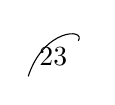
\begin{tikzpicture}[baseline=(p.base)]
\node[inner sep=1pt] (p) {23};
\draw ([xshift=-1mm,yshift=-1mm]p.south west) .. controls ([xshift=1mm,yshift=2mm]p.north west) and ([xshift=2mm,yshift=2mm]p.north east) .. ([xshift=1mm,yshift=.4mm]p.north east);
\end{tikzpicture}}}
% archive sheet number: 39 (inverted, upper left)
% Top and bottom continuations retain their physical marginal positions and their paired call marks.
\inserted{\handwritten{\figure{\begin{tikzpicture}
\node[inner sep=5pt,text width=.96\linewidth,align=left] (top) {
\tikz[baseline=-.4ex,x=1ex,y=1ex]{\draw[line width=.45pt] (.15,1.5)--(.15,.38);\draw[line width=.4pt] (.15,.12) ellipse (.16 and .24);\fill (.15,.37) ellipse (.12 and .14);}
\begin{tikzpicture}[baseline=(op.base)]
\node[inner sep=0pt] (op) {opérations};
\node[anchor=south west,inner sep=0pt] at ([xshift=-.35em,yshift=-.3ex]op.north west) {les};
% The pale rising trace has no assigned alphabetic or editorial function.
\node[inner sep=0pt] at ([xshift=.4em]op.north west) {\unsure{\begin{tikzpicture}[overlay,x=1em,y=1ex]
\draw[gray,line width=.3pt] (-.6,-.65)--(-.6,-.2) .. controls (-.05,.4) and (.6,.9) .. (.9,1.8);
\end{tikzpicture}}};
\end{tikzpicture}
fonctorielles \deleted{\illegible{1}} habituelles faites en termes de telles structures, plus précisément à toutes les opérations qui
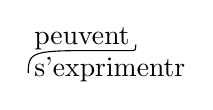
\begin{tikzpicture}[baseline=(expr.base)]
\node[inner sep=0pt] (expr) {s'exprime\deleted{nt}\unsure{r}};
\node[anchor=south west,inner sep=0pt] (peuvent) at ([yshift=.5ex]expr.north west) {\inserted{peuvent}};
\draw ([xshift=-.2em,yshift=-.3ex]expr.west) .. controls ([xshift=-.2em,yshift=.7ex]expr.north west) and (peuvent.south west) .. (peuvent.south east) .. controls ([xshift=.2em]peuvent.south east) .. ([xshift=.2em,yshift=.5ex]peuvent.south east);
\end{tikzpicture}
en termes de $\varinjlim$ et de $\varprojlim$ finies: constructions d'objets libres (groupes ou modules libres, p.ex.) engendrés par un objet, produits tensoriels (cf. \S 6 plus bas) etc.};
\draw ([yshift=2mm]top.north west) .. controls ([xshift=-1mm]top.west) and ([xshift=-1mm]top.south west) .. (top.south west) -- (top.south) -- ([yshift=2mm]top.south) -- ([yshift=2mm]top.south east);
\end{tikzpicture}}}}

sent en termes de limites projectives finies exclusivement, tandis que les autres notions impliquent implicitement des constructions faisant appel également à des limites inductives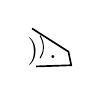
\begin{tikzpicture}[baseline=(close.base)]
\node[inner sep=0pt] (close) {)};
\node[anchor=base west,inner sep=0pt] (trace) at (close.base east) {\handwritten{\unsure{\tikz[baseline=-.35ex,x=1ex,y=1ex]{\draw[line width=.35pt] (0,1.6) .. controls (.4,.9) and (.35,.2) .. (0,-.3);}}}};
\node[anchor=base west,inner sep=0pt] (stop) at ([xshift=.1em]trace.base east) {.};
\draw[line width=.6pt] ([xshift=-.25em,yshift=.5ex]trace.north west)--([xshift=.4em,yshift=.3ex]stop.north east)--([xshift=.5em,yshift=-.5ex]stop.south east)--([xshift=-.1em,yshift=-.6ex]trace.south west);
\end{tikzpicture}

% Slanted marginal paragraphing instruction; the enclosure is open at the left.
\margin{\handwritten{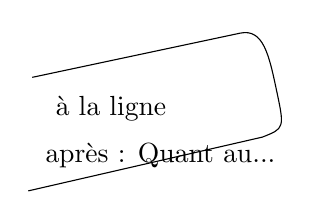
\begin{tikzpicture}[rotate=12]
\node[anchor=west,inner sep=0pt] (line) at (.1,.55) {à la ligne};
\node[anchor=west,inner sep=0pt] (apres) at (-.15,0) {après : Quant au...};
\draw (-.1,1)--(2.6,1) .. controls (2.9,1) and (2.9,.65) .. (2.9,.2) .. controls (2.9,-.3) .. (2.6,-.35)--(-.45,-.4);
\end{tikzpicture}}}
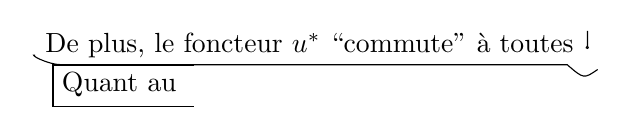
\begin{tikzpicture}[baseline=(quant.base)]
\node[inner sep=1pt,anchor=base west] (quant) at (0,0) {Quant au};
\node[anchor=south west,inner sep=1pt] (plus) at ([xshift=-.6em,yshift=.7ex]quant.north west) {\inserted{\handwritten{De plus, le foncteur $u^{*}$ ``\uline{commute}'' à toutes
\tikz[baseline=-.35ex,x=1ex,y=1ex]{\draw (.12,1.45)--(.12,.2) .. controls (-.22,-.08) and (.42,-.08) .. (.12,.2);}}}};
\draw ([xshift=-.25em,yshift=.5ex]plus.south west) .. controls ([xshift=-.5em,yshift=.6ex]plus.south west) and ([xshift=.2em,yshift=-.3ex]plus.south west) .. ([xshift=.7em,yshift=-.3ex]plus.south west)
-- ([xshift=-1em,yshift=-.3ex]plus.south east) .. controls ([xshift=-.4em,yshift=-1.5ex]plus.south east) .. ([xshift=.1em,yshift=-.7ex]plus.south east);
\draw[line width=.6pt] ([xshift=.5em,yshift=.4ex]quant.north east)--([xshift=-.2em,yshift=.4ex]quant.north west)--([xshift=-.2em,yshift=-.5ex]quant.south west)--([xshift=.5em,yshift=-.5ex]quant.south east);
\end{tikzpicture}
foncteur image directe
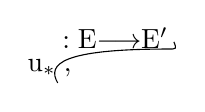
\begin{tikzpicture}[baseline=(direct.base)]
\node[inner sep=0pt] (direct) {$\mathrm{u}_{\handwritten{*}}$};
\node[anchor=base west,inner sep=0pt] (comma) at ([xshift=.25em]direct.base east) {,};
\node[anchor=south west,inner sep=0pt] (map) at ([xshift=.2em,yshift=.8ex]direct.north east) {\inserted{$:\mathrm{E}\handwritten{\longrightarrow}\mathrm{E}'$}};
\handwritten{\draw ([xshift=-.2em,yshift=-.5ex]comma.south west) .. controls ([xshift=-.6em,yshift=.7ex]comma.west) and (map.south west) .. (map.south east) .. controls ([xshift=.3em]map.south east) .. ([xshift=.2em,yshift=.6ex]map.south east);}
\end{tikzpicture}
qui commute aux limites projectives, il ``respecte''
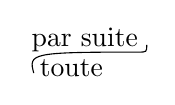
\begin{tikzpicture}[baseline=(toute.base)]
\node[inner sep=0pt] (toute) {toute};
\node[anchor=south west,inner sep=0pt] (suite) at ([xshift=-.3em,yshift=.6ex]toute.north west) {\inserted{par suite}};
\handwritten{\draw ([xshift=-.2em,yshift=-.4ex]toute.west) .. controls ([xshift=-.4em,yshift=.5ex]toute.north west) and (suite.south west) .. (suite.south east) .. controls ([xshift=.3em]suite.south east) .. ([xshift=.3em,yshift=.6ex]suite.south east);}
\end{tikzpicture}
structure algébrique sur un objet (ou une famille d'objets) de $\mathrm{E}$, définissable en termes de limites projectives
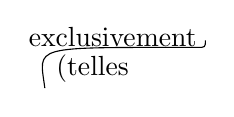
\begin{tikzpicture}[baseline=(telles.base)]
\node[inner sep=0pt] (telles) {(telles};
\node[anchor=south west,inner sep=0pt] (excl) at ([xshift=-1em,yshift=.6ex]telles.north west) {\inserted{exclusivement}};
\handwritten{\draw ([xshift=-.4em,yshift=-.4ex]telles.south west) .. controls ([xshift=-.6em,yshift=.8ex]telles.north west) and (excl.south west) .. (excl.south east) .. controls ([xshift=.3em]excl.south east) .. ([xshift=.3em,yshift=.6ex]excl.south east);}
\end{tikzpicture}
les structures de groupe, d'anneau ou de module sur un anneau, 
\begin{tikzpicture}[baseline=(dans.base)]
\node[inner sep=0pt] (dans) {\deleted{dans}};
\node[anchor=south west,inner sep=0pt] at ([yshift=-.35ex]dans.north west) {\inserted{parmi}};
\end{tikzpicture} les exemples précédents). Par
\unsure{
\begin{tikzpicture}[baseline=(c.base)]\node[inner sep=0pt] (c) {c};\node[inner sep=0pt] at ([xshift=.05ex]c.center) {f};\end{tikzpicture}}ontre,
le foncteur $\mathrm{u}_{\handwritten{*}}$ n\deleted{e}'est en général pas exact à droite i.e. il ne commute pas en général aux limites inductives finies, et même ne transforme pas en général épimorphisme en épimorphisme
\handwritten{\unsure{
\begin{tikzpicture}[baseline=-.2ex,x=1ex,y=1ex]
\draw[line width=.5pt] (.14,-.3) .. controls (-.18,-.2) and (.02,.35) .. (.2,.6) .. controls (.38,1.1) and (.1,1.7) .. (.35,2.15);
\draw[line width=.7pt] (.18,.35) ellipse (.13 and .25);
\draw[line width=.5pt] (.47,2.25)--(.6,2.35)--(.68,2.15);
\end{tikzpicture}}(}
c'est d'ailleurs
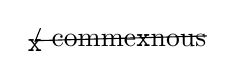
\begin{tikzpicture}[baseline=(del.base)]
\node[inner sep=0pt] (del) {\deleted{\unsure{comme}}\tikz[baseline=(x.base)]{\node[inner sep=0pt] (x) {\texttt{x}};}\deleted{nous}};
\node[anchor=base east,inner sep=0pt] (blankx) at ([xshift=-.3em,yshift=-.4ex]del.base west) {\texttt{x}};
\handwritten{\draw ([yshift=.4ex]blankx.center)--([yshift=.4ex]del.east);\draw ([yshift=.3ex]blankx.center)--([xshift=.2em,yshift=.9ex]blankx.north);}
\end{tikzpicture}
\tikz[baseline=(x.base)]{\node[inner sep=0pt] (x) {\texttt{x}};}\deleted{le}\tikz[baseline=(x.base)]{\node[inner sep=0pt] (x) {\texttt{x}};}\deleted{verrons}\tikz[baseline=(x.base)]{\node[inner sep=0pt] (x) {\texttt{x}};}\deleted{au}
ce défaut d'exactitude du foncteur $\mathrm{u}_{\handwritten{*}}$ qui est \begin{tikzpicture}[baseline=(a.base)]
\node[inner sep=0pt] (a) {\handwritten{à}};
\node[inner sep=0pt] at (a.north west) {\unsure{\begin{tikzpicture}[overlay,x=1ex,y=1ex]
\draw[gray,line width=.25pt] (.1,2.2) .. controls (.02,1.5) and (.02,.8) .. (-.05,.25);
\draw[gray,line width=.25pt] (-.05,.1)--(.08,-.4);
\end{tikzpicture}}};
\end{tikzpicture} la source de ces propriétés cohomologiques, qui seront étudiées (du point de vue de l'algèbre homologique commutative) dans l'exposé suivant\handwritten{)}.
\inserted{\handwritten{Par suite, il ne
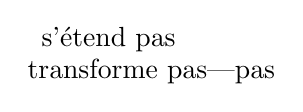
\begin{tikzpicture}[baseline=(old.base)]
\node[inner sep=0pt] (old) {\deleted{\unsure{transforme}} \unsure{pas|\deleted{pas}}};
\node[anchor=south west,inner sep=0pt] at ([xshift=.5em,yshift=.5ex]old.north west) {\inserted{s'étend pas}};
\end{tikzpicture}, en général,
\tikz[baseline=-.3ex,x=1ex,y=1ex]{\draw (0,-.2)--(.12,1.3);\draw (.12,1.4) ellipse (.14 and .12);}}}

\deleted{2}\handwritten{3}.1.3. En pratique, lorsqu'on
\begin{tikzpicture}[baseline=(un.base)]
\node[inner sep=0pt,anchor=base west] (se) at (0,0) {\deleted{se}\tikz[baseline=(x.base)]{\node[inner sep=0pt] (x) {\texttt{x}};}\deleted{donne}};
\node[anchor=base west,inner sep=0pt] (un) at ([xshift=.3em]se.base east) {un};
\node[anchor=south west,inner sep=0pt] (presence) at ([xshift=-.3em,yshift=.8ex]se.north west) {\inserted{\begin{tikzpicture}[baseline=(estp.base)]
\node[inner sep=0pt] (estp) {est};
\node[anchor=base west,inner sep=0pt] at ([xshift=.6em]estp.base east) {présenced'};
\node[anchor=south west,inner sep=0pt] at ([xshift=.1em,yshift=-.3ex]estp.north east) {\inserted{\handwritten{en}}};
\end{tikzpicture}}};
\handwritten{\draw ([xshift=-.2em,yshift=-.4ex]un.south west) .. controls ([xshift=-.2em,yshift=.7ex]un.north west) and (presence.south west) .. (presence.south east) .. controls ([xshift=.3em]presence.south east) .. ([xshift=.3em,yshift=.6ex]presence.south east);}
\end{tikzpicture}
foncteur $\mathrm{f}:\mathrm{E}\handwritten{\longrightarrow}\mathrm{F}$ d'un $\underline{\mathrm{U}}$-topos dans un autre, il y a lieu d'en expliciter
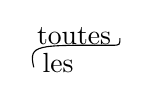
\begin{tikzpicture}[baseline=(les.base)]
\node[inner sep=0pt] (les) {les};
\node[anchor=south west,inner sep=0pt] (toutes) at ([xshift=-.2em,yshift=.6ex]les.north west) {\inserted{\handwritten{toutes}}};
\handwritten{\draw ([xshift=-.3em,yshift=-.4ex]les.west) .. controls ([xshift=-.5em,yshift=.7ex]les.north west) and (toutes.south west) .. (toutes.south east) .. controls ([xshift=.3em]toutes.south east) .. ([xshift=.3em,yshift=.6ex]toutes.south east);}
\end{tikzpicture}
propri\unsure{
\begin{tikzpicture}[baseline=(e.base)]\node[inner sep=0pt] (e) {é};\node[inner sep=0pt] at (e.center) {t};\end{tikzpicture}}\unsure{
\begin{tikzpicture}[baseline=(t.base)]\node[inner sep=0pt] (t) {t};\node[inner sep=0pt] at (t.center) {é};\end{tikzpicture}}és d'exactitude,
% The x impressions in spaces are cancellation marks, not underlying prose.
\deleted{y}\tikz[baseline=(x.base)]{\node[inner sep=0pt] (x) {\texttt{x}};}\deleted{compris}\tikz[baseline=(x.base)]{\node[inner sep=0pt] (x) {\texttt{x}};}\deleted{et}\tikz[baseline=(x.base)]{\node[inner sep=0pt] (x) {\texttt{x}};}\deleted{de}\tikz[baseline=(x.base)]{\node[inner sep=0pt] (x) {\texttt{x}};}\deleted{déterminer}\tikz[baseline=(x.base)]{\node[inner sep=0pt] (x) {\texttt{x}};}\deleted{s'il}\tikz[baseline=(x.base)]{\node[inner sep=0pt] (x) {\texttt{x}};}\deleted{admet}\tikz[baseline=(x.base)]{\node[inner sep=0pt] (x) {\texttt{x}};}\deleted{un}\tikz[baseline=(x.base)]{\node[inner sep=0pt] (x) {\texttt{x}};}\deleted{foncteur}\tikz[baseline=(x.base)]{\node[inner sep=0pt] (x) {\texttt{x}};}\deleted{exact}
y compris l'existence éventuelle de foncteurs adjoints à gauche ou à droite (cf. la note de bas de page précédente), pour parvenir à une compréhension de la ``nature géométrique'' de $\mathrm{f}$, \deleted{qui} compréhension qui sera généralement un guide indispensable pour
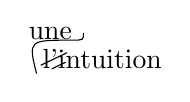
\begin{tikzpicture}[baseline=(intuition.base)]
\node[inner sep=0pt] (intuition) {\deleted{l'}intuition};
\node[anchor=south west,inner sep=0pt] (une) at ([xshift=-.5em,yshift=.7ex]intuition.north west) {\inserted{une}};
\handwritten{\draw ([xshift=-.2em,yshift=-.4ex]intuition.south west) .. controls ([xshift=-.5em,yshift=.7ex]intuition.north west) and (une.south west) .. (une.south east) .. controls ([xshift=.4em]une.south east) .. ([xshift=.4em,yshift=.6ex]une.south east);}
\handwritten{
\draw[line width=.4pt] ([xshift=-.05em,yshift=.25ex]intuition.base west)--([xshift=.9em,yshift=1.3ex]intuition.base west);
\draw[line width=.4pt] ([xshift=.35em,yshift=-.05ex]intuition.base west)--([xshift=.85em,yshift=.5ex]intuition.base west);}
\end{tikzpicture}
géométrique correcte de la situation. Ainsi, s'il s'avère que $\mathrm{f}$ commute aux limites inductives quelconques et aux limites projectives finies, il y a lieu d'écrire $\mathrm{f}$ sous la forme
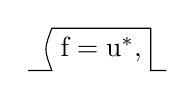
\begin{tikzpicture}[baseline=(f.base)]\node[inner sep=3pt] (f) {$\mathrm{f}=\mathrm{u}^{\handwritten{*}}$,};\handwritten{\draw ([xshift=-3mm]f.south west)--(f.south west) .. controls ([xshift=-1mm]f.west) .. (f.north west)--(f.north east)--(f.south east)--([xshift=2mm]f.south east);}\end{tikzpicture}
où
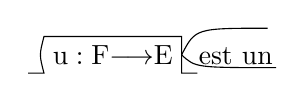
\begin{tikzpicture}[baseline=(u.base)]
\node[inner sep=3pt] (u) {$\mathrm{u}:\mathrm{F}\handwritten{\longrightarrow}\mathrm{E}$};
\node[anchor=base west,inner sep=1pt] (est) at ([xshift=.5em]u.base east) {est un};
\handwritten{\draw ([xshift=-2mm]u.south west)--(u.south west) .. controls ([xshift=-.6mm]u.west) .. (u.north west)--(u.north east)--(u.south east)--([xshift=2mm]u.south east);
\draw (u.east) .. controls ([yshift=2mm]est.north west) .. ([xshift=-.3em,yshift=2mm]est.north east);
\draw (u.east) .. controls (est.south west) .. (est.south east);}
\end{tikzpicture}
morphisme de topos, i.e. d'interpréter $\mathrm{f}$ comme un foncteur ``image inverse'' par une ````application continue'' de topos.
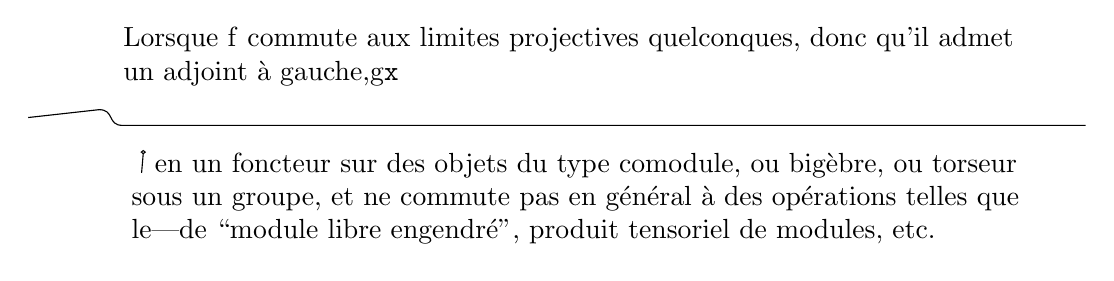
\begin{tikzpicture}
\node[anchor=north west,inner sep=0pt,text width=.96\linewidth,align=left] (last) at (0,0) {Lorsque $\mathrm{f}$ commute aux limites projectives quelconques, donc qu'il admet un adjoint à gauche,\deleted{$\mathrm{g}$}\tikz[baseline=(x.base)]{\node[inner sep=0pt] (x) {\texttt{x}};}};
\node[anchor=north west,inner sep=3pt,text width=.99\linewidth,align=left] (bottom) at ([yshift=-7mm]last.south west) {\inserted{\handwritten{
\tikz[baseline=-.3ex,x=1ex,y=1ex]{\draw (0,-.35)--(.14,1.3);\draw (.14,1.4) ellipse (.16 and .13);}
en un foncteur sur des objets du type comodule, ou bigèbre, ou torseur sous un groupe\unsure{,} et ne commute pas en général à des opérations telles que \deleted{\unsure{le|de}} ``module libre engendré'', produit tensoriel de modules, etc.}}};
\handwritten{\draw ([xshift=-12mm,yshift=3mm]bottom.north west)--([xshift=-3mm,yshift=4mm]bottom.north west) .. controls ([xshift=-1mm,yshift=4mm]bottom.north west) and ([xshift=-2mm,yshift=2mm]bottom.north west) .. ([yshift=2mm]bottom.north west)--([yshift=2mm]bottom.north east);}
\end{tikzpicture}
